\documentclass{exam}
\usepackage{ctex}
\usepackage{tikz}
\usepackage{amsmath}
\title{Discrete Mathematics for Computer Science Spring 2023\\
       Final}
\date{June 8, 2023}
\author{514B}
\begin{document}
\maketitle
\part{选择题}
\begin{questions}
    \question[5]非连通图$G$有7个顶点, 最多有多少条边?
    \begin{oneparchoices}
        \choice 7
        \choice 15
        \choice 21
    \end{oneparchoices}
    \question[5]$2n$个顶点的树最多有多少个完全匹配?
    \begin{oneparchoices}
        \choice $0$
        \choice $1$
        \choice $n-1$
        \choice $n$
    \end{oneparchoices}
    \question[5]有以下字符及其出现概率: 0: 30\%, 1:20\%, 2: 15\%, 3: 10\%, 4: 10\%, 5: 6\%, 6: 5\%, 7: 4\%. 请问若使编码长度最小, 10000个字符的预期编码长度为多少?
    \begin{oneparchoices}
        \choice 20000
        \choice 20900
        \choice 27400
        \choice 29600
    \end{oneparchoices}
    \question[5]下列说法正确的个数是: \\
    (1). 字符串aX, Xb, aZ, tZ , 能否找到某种方法, 使用6个字母排出这5个字符串首尾相接(不考虑顺序, 即aX与Xa均可)的拼接结果. \\
    (2). 一个有6个顶点, 12条边的平面图, 它的每个域的边界数均为3. \\
    (3). 下图有H回路. \\
    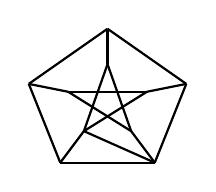
\begin{tikzpicture}
        \draw[black, thick](-0.5,0)--(0.5,0);
        \draw[black, thick](0.5,0)--(-0.3,-0.5);
        \draw[black, thick](-0.3,-0.5)--(0,0.35);
        \draw[black, thick](0,0.35)--(0.3,-0.5);
        \draw[black, thick](0.3,-0.5)--(-0.5,0);
        \draw[black, thick](-0.5,0)--(-1,0.1);
        \draw[black, thick](0.5,0)--(1,0.1);
        \draw[black, thick](0,0.35)--(0,0.8);
        \draw[black, thick](-0.3,-0.5)--(-0.6,-0.9);
        \draw[black, thick](0.3,-0.5)--(0.6,-0.9);
        \draw[black, thick](-0.3,-0.5)--(0.6,-0.9);
        \draw[black, thick](0.6,-0.9)--(-0.6,-0.9);
        \draw[black, thick](1,0.1)--(0.6,-0.9);
        \draw[black, thick](-1,0.1)--(-0.6,-0.9);
        \draw[black, thick](1,0.1)--(0,0.8);
        \draw[black, thick](-1,0.1)--(0,0.8);
    \end{tikzpicture}
    \\
    \begin{oneparchoices}
        \choice 1
        \choice 2
        \choice 3
        \choice 4
    \end{oneparchoices}
\end{questions}
\part{填空题}
\begin{questions}
    \question 字符串ac, bd, abe, ad, ce, 找到它们与字母a$\sim$e的一一对应.
    \question 求下图所有的最小生成树. (图没记住
    \question 有21个人, 围成一个圆圈坐, 每轮要求与之前所有轮的相邻者不同, 问最多可以进行多少轮.
    \question 有一系列无向图$G_n$, 由$n+1$个顶点组成, 结构为一个核心节点连接剩余$n$个节点, 剩余$n$个节点形成一个环. 比如$G_4$: 
    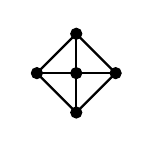
\begin{tikzpicture}
        \filldraw[black](0,0)circle(2pt)node[anchor=north]{};
        \filldraw[black](-0.5,0)circle(2pt)node[anchor=north]{};
        \filldraw[black](0.5,0)circle(2pt)node[anchor=north]{};
        \filldraw[black](0,0.5)circle(2pt)node[anchor=north]{};
        \filldraw[black](0,-0.5)circle(2pt)node[anchor=north]{};
        \draw[black, thick](-0.5,0)--(0.5,0);
        \draw[black, thick](0,-0.5)--(0,0.5);
        \draw[black, thick](-0.5,0)--(0,0.5);
        \draw[black, thick](-0.5,0)--(0,-0.5);
        \draw[black, thick](0.5,0)--(0,0.5);
        \draw[black, thick](0.5,0)--(0,-0.5);
    \end{tikzpicture}
    . 尝试求出$G_4$的树的数目以及$G_n$的树的数目的递推公式.
\end{questions}
\part{解答题}
\begin{questions}
    \question 有某个无向图(图没记住), 求 \\
    (1). 该图的中国邮路; \\
    (2). 该图是否可平面? 最小覆盖数是多少? 其色相多项式是多少? \\
    \question (1). 证明$S_e C_e^T=0$; \\
    (2). 已知图$G$的关联矩阵$B=
    \begin{bmatrix}
        1 & 1 & 0 & 0 & 0 & 0 & 0 \\
        0 & -1 & 1 & 0 & 1 & 1 & 0 \\
        0 & 0 & 0 & 0 & 0 & -1 & -1 \\
        -1 & 0 & 0 & -1 & -1 & 0 & 1 \\
        0 & 0 & -1 & 1 & 0 & 0 & 0 \\
    \end{bmatrix}$
    , 画出图$G$, 写出$C_f$, 并计算$S_f$.
    \question 证明五色定理.
    \question 证明$\sum(d^+(v_i))^2=\sum(d^-(v_i))^2$.
\end{questions}
\end{document}